\documentclass[a4paper, UTF-8]{article}
\usepackage{algorithm}
\usepackage{algpseudocode}
\usepackage{amsmath}
\usepackage{amsfonts}
\usepackage{amsthm}
\usepackage{tikz}
\usetikzlibrary{automata, positioning, arrows}
\usepackage[utf8]{inputenc} % allow utf-8 input
\usepackage[T1]{fontenc}    % use 8-bit T1 fonts
\usepackage{hyperref}       % hyperlinks
\usepackage{url}            % simple URL typesetting
\usepackage{booktabs}       % professional-quality tables
\usepackage{amsfonts}       % blackboard math symbols
\usepackage{nicefrac}       % compact symbols for 1/2, etc.
\usepackage{microtype}      % microtypography
\usepackage{xcolor}         % colors

\theoremstyle{plain}
\newtheorem{theorem}{\indent Theorem}[section]
\newtheorem{lemma}[theorem]{\indent Lemma}
\newtheorem{assumption}{\indent Assumption}[section]
\newtheorem{note}[theorem]{\indent Notation}
\newtheorem{proposition}[theorem]{\indent Proposition}
\newtheorem{corollary}[theorem]{\indent Corollary}
\newtheorem{definition}{\indent Definition}[section]
\newtheorem{example}{\indent Example}[section]
\newtheorem{remark}{\indent Remark}[section]
\newenvironment{solution}{\begin{proof}[\indent\bf Solution]}{\end{proof}}
\renewcommand{\proofname}{\indent\bf Proof}

\begin{document}

\title{\bf{Lab1 Answers}}

\author{Yanqiao Chen*\\ 
  Department of Computer Science and Engineering\\
  Southern University of Science and Technology\\
  \texttt{12412115@mail.sustech.edu.cn}
  }

\maketitle

\section{Question 1}

\begin{enumerate}
    \item [a.] $Q_1 =\{ q_1 \}$, $Q_2 = \{q_1\}$
    \item [b.] $F_1 = \{q_2\}$, $F_2 = \{q_1, q_4\}$
    \item [c.] $M_1: q_1 \to q_2 \to q_3 \to q_1 \to q_1$, $M_2: q_1 \to q_1 \to q_1 \to q_2 \to q_4$.
    \item [d.] $M_1: No$, $M_2: Yes$.
    \item [e.] $M_1: No$, $M_2: Yes$
\end{enumerate}

\section{Question 2}

$M_1$ for Q1 can be described as the following DFA:

\begin{itemize}
    \item States: $Q = \{q_1, q_2, q_3\}$
    \item Alphabet: $\Sigma = \{a, b\}$
    \item Transition function: 
            \begin{center}
              \begin{tabular}{c|c|c}
                  $\delta$ & $a$ & $b$ \\
                  \hline
                  $q_1$ & $q_2$ & $q_1$ \\
                  $q_2$ & $q_3$ & $q_3$ \\
                  $q_3$ & $q_2$ & $q_1$
              \end{tabular}
            \end{center}
    \item Initial state: $q_1$
    \item Accepting states: $F = \{q_2\}$
\end{itemize}

\newpage

$M_2$ for Q1 can be described as the following DFA:

\begin{itemize}
    \item States: $Q = \{q_1, q_2, q_3, q_4\}$
    \item Alphabet: $\Sigma = \{a, b\}$
    \item Transition function: 
            \begin{center}
              \begin{tabular}{c|c|c}
                  $\delta$ & $a$ & $b$ \\
                  \hline
                  $q_1$ & $q_1$ & $q_2$ \\
                  $q_2$ & $q_3$ & $q_4$ \\
                  $q_3$ & $q_2$ & $q_1$ \\ 
                  $q_4$ & $q_3$ & $q_4$
              \end{tabular}
            \end{center}
    \item Initial state: $q_1$
    \item Accepting states: $F = \{q_1, q_4\}$

\end{itemize}

\section{Question 3}

\begin{center}
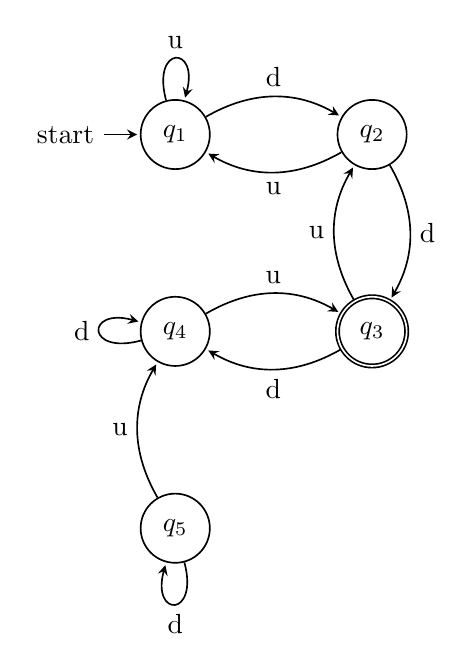
\begin{tikzpicture}[->,>=stealth,shorten >=1pt,auto,node distance=2.5cm, semithick]
  \node[state,initial] (q1) {$q_1$};
  \node[state] (q2) [right of=q1] {$q_2$};
  \node[state,accepting] (q3) [below of=q2] {$q_3$};
  \node[state] (q4) [left of=q3] {$q_4$};
  \node[state] (q5) [below of=q4] {$q_5$};

  \path (q1) edge [loop above] node {u} (q1)
        (q1) edge [bend left] node {d} (q2)
        (q2) edge [bend left] node {u} (q1)
        (q2) edge [bend left] node {d} (q3)
        (q3) edge [bend left] node {u} (q2)
        (q3) edge [bend left] node {d} (q4)
        (q4) edge [bend left] node {u} (q3)
        (q4) edge [loop left] node {d} (q5)
        (q5) edge [bend left] node {u} (q4)
        (q5) edge [loop below] node {d} (q5);
\end{tikzpicture}
\end{center}

\section{Question 4} 

\subsection{a}

\begin{center}
    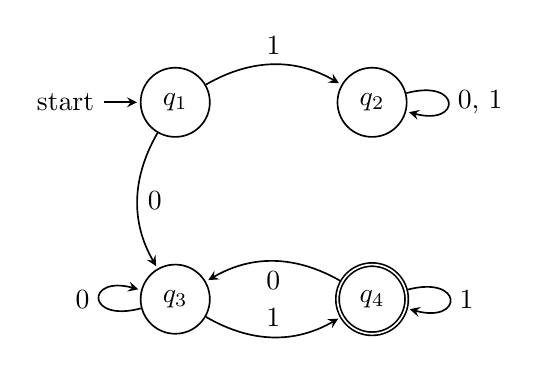
\begin{tikzpicture}[->,>=stealth,shorten >=1pt,auto,node distance=2.5cm, semithick]
      \node[state,initial] (q1) {$q_1$};
      \node[state] (q2) [right of=q1] {$q_2$};
      \node[state] (q3) [below of=q1] {$q_3$};
      \node[state,accepting] (q4) [below of=q2] {$q_4$};

      \path (q1) edge [bend left] node {1} (q2)
            (q2) edge [loop right] node {0, 1} (q2)
            (q1) edge [bend right] node {0} (q3)
            (q3) edge [bend right] node {1} (q4)
            (q4) edge [bend right] node {0} (q3)
            (q4) edge [loop right] node {1} (q4)
            (q3) edge [loop left] node {0} (q3);
    \end{tikzpicture}
\end{center}

\subsection{b} 

\begin{center}
    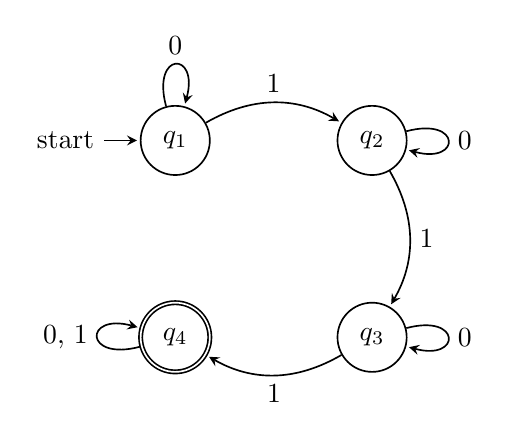
\begin{tikzpicture}[->,>=stealth,shorten >=1pt,auto,node distance=2.5cm, semithick]
      \node[state,initial] (q1) {$q_1$};
      \node[state] (q2) [right of=q1] {$q_2$};
      \node[state, accepting] (q4) [below of=q1] {$q_4$};
      \node[state] (q3) [below of=q2] {$q_3$};

      \path (q1) edge [bend left] node {1} (q2)
            (q1) edge [loop above] node {0} (q1)
            (q2) edge [bend left] node {1} (q3)
            (q2) edge [loop right] node {0} (q2)
            (q3) edge [bend left] node {1} (q4)
            (q3) edge [loop right] node {0} (q3)
            (q4) edge [loop left] node {0, 1} (q4)
            ;
            
    \end{tikzpicture}
\end{center}

\subsection{c}

\begin{center}
    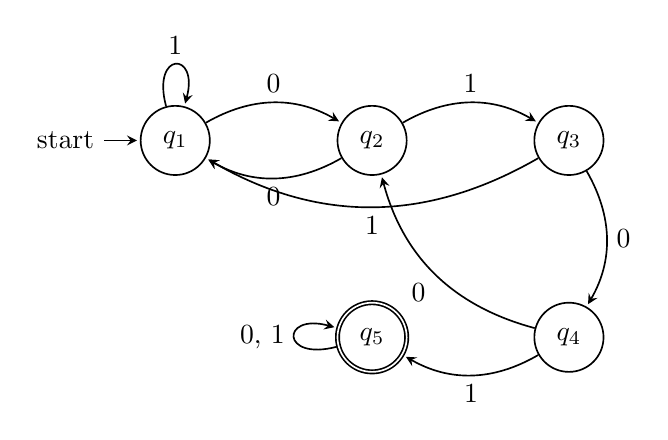
\begin{tikzpicture}[->,>=stealth,shorten >=1pt,auto,node distance=2.5cm, semithick]
      \node[state,initial] (q1) {$q_1$};
      \node[state] (q2) [right of=q1] {$q_2$};         
      \node[state] (q3) [right of=q2] {$q_3$};
      \node[state, accepting] (q5) [below of=q2] {$q_5$};
      \node[state] (q4) [below of=q3] {$q_4$};


      \path (q1) edge [bend left] node {0} (q2)
            (q1) edge [loop above] node {1} (q1)
            (q2) edge [bend left] node {1} (q3)
            (q2) edge [bend left] node {0} (q1)
            (q3) edge [bend left] node {0} (q4)
            (q3) edge [bend left] node {1} (q1)
            (q4) edge [bend left] node {1} (q5)
            (q4) edge [bend left] node {0} (q2)
            (q5) edge [loop left] node {0, 1} (q5)
            ;
            
    \end{tikzpicture}
\end{center}



\subsection{d}

\begin{center}
    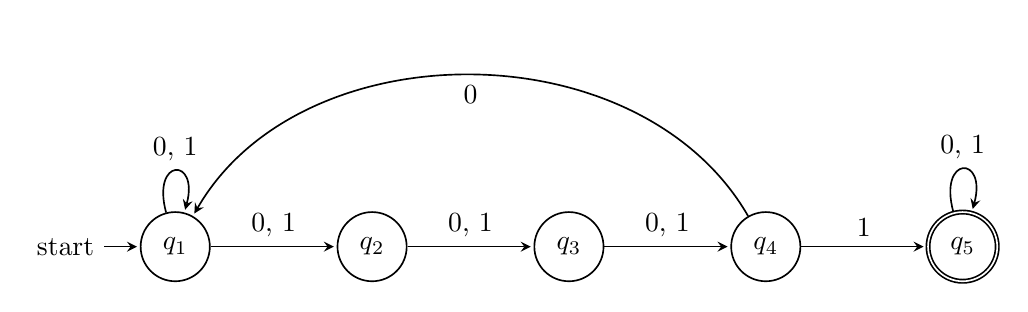
\begin{tikzpicture}[->,>=stealth,shorten >=1pt,auto,node distance=2.5cm, semithick]
      \node[state,initial] (q1) {$q_1$};
      \node[state] (q2) [right of=q1] {$q_2$};
      \node[state] (q3) [right of=q2] {$q_3$};
      \node[state] (q4) [right of=q3] {$q_4$};
      \node[state, accepting] (q5) [right of=q4] {$q_5$};

      \path (q1) edge [loop above] node {0, 1} (q1)
            (q1) edge node {0, 1} (q2)
            (q2) edge node {0, 1} (q3)
            (q3) edge node {0, 1} (q4)
            (q4) edge node {1} (q5)
            (q4) edge [bend right=60] node[below] {0} (q1)
            (q5) edge [loop above] node {0, 1} (q5)
            ;
    \end{tikzpicture}
\end{center}

\subsection{e}

\begin{center}
    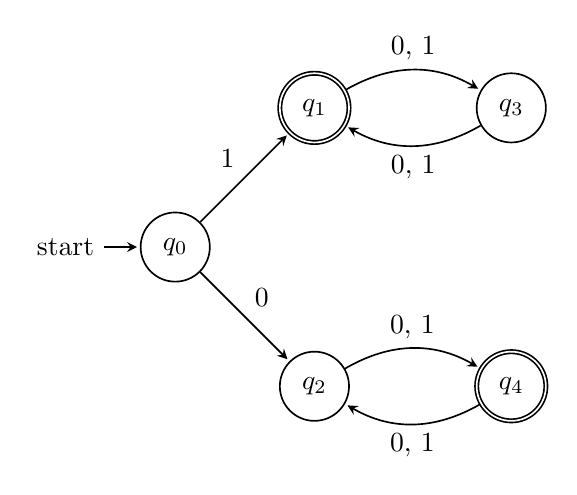
\begin{tikzpicture}[->,>=stealth,shorten >=1pt,auto,node distance=2.5cm, semithick]
      \node[state,initial] (q0) {$q_0$};
      \node[state, accepting] (q1) [above right of=q0] {$q_1$};
      \node[state] (q2) [below right of=q0] {$q_2$};
      \node[state] (q3) [right of=q1] {$q_3$};
      \node[state, accepting] (q4) [right of=q2] {$q_4$};

      \path (q0) edge node {1} (q1)
            (q0) edge node {0} (q2)
            (q1) edge [bend left] node {0, 1} (q3)
            (q2) edge [bend left] node {0, 1} (q4)
            (q3) edge [bend left] node {0, 1} (q1)
            (q4) edge [bend left] node {0, 1} (q2)
            ;
    \end{tikzpicture}
\end{center}

\subsection{f}

\begin{center}
    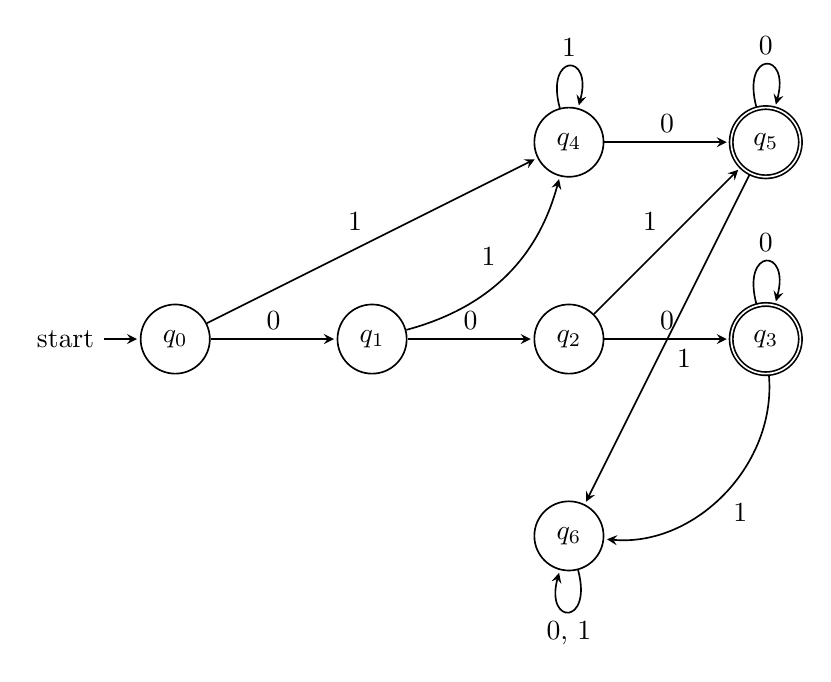
\begin{tikzpicture}[->,>=stealth,shorten >=1pt,auto,node distance=2.5cm, semithick]
      \node[state,initial] (q0) {$q_0$};
      \node[state] (q1) [right of=q0] {$q_1$};
      \node[state] (q2) [right of=q1] {$q_2$};
      \node[state, accepting] (q3) [right of=q2] {$q_3$};
      \node[state] (q4) [above of=q2] {$q_4$};
      \node[state, accepting] (q5) [right of=q4] {$q_5$};
      \node[state] (q6) [below of=q2] {$q_6$};

      \path (q0) edge node {0} (q1)
            (q0) edge node {1} (q4)
            (q1) edge node {0} (q2)
            (q1) edge [bend right] node {1} (q4)
            (q2) edge node {0} (q3)
            (q2) edge node {1} (q5)
            (q3) edge [loop above] node {0} (q3)
            (q3) edge [bend left=50] node {1} (q6)
            (q4) edge node {0} (q5)
            (q4) edge [loop above] node {1} (q6)
            (q5) edge [loop above] node {0} (q5)
            (q5) edge node {1} (q6)
            (q6) edge [loop below] node {0, 1} (q6)
            ;
    \end{tikzpicture}
\end{center}

\subsection{g}

\begin{center}
    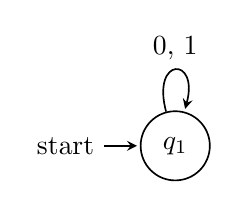
\begin{tikzpicture}[->,>=stealth,shorten >=1pt,auto,node distance=2.5cm, semithick]
      \node[state,initial] (q1) {$q_1$};

      \path (q1) edge [loop above] node {0, 1} (q1)
            ;
    \end{tikzpicture}
\end{center}

\subsection{h}

\begin{center}
    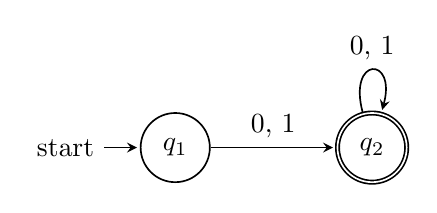
\begin{tikzpicture}[->,>=stealth,shorten >=1pt,auto,node distance=2.5cm, semithick]
      \node[state,initial] (q1) {$q_1$};
      \node[state, accepting] (q2) [right of=q1] {$q_2$};

      \path (q1) edge node {0, 1} (q2)
            (q2) edge [loop above] node {0, 1} (q2)
            ;
    \end{tikzpicture}
\end{center}

\section{Question 5} 

For each language, we first construct a DFA for the simpler language, then swap accepting and non-accepting states to get the DFA for the original language.

\subsection{a) $\{w \mid w \text{ does not contain the substring } ba\}$}

The simpler language is $\{w \mid w \text{ contains the substring } ba\}$.

DFA for the simpler language (contains $ba$):
\begin{center}
    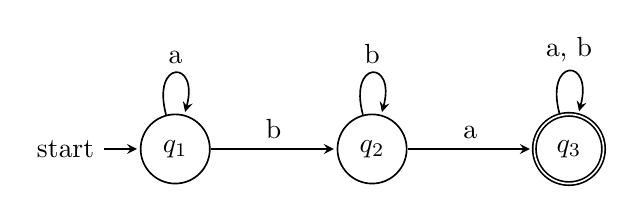
\begin{tikzpicture}[->,>=stealth,shorten >=1pt,auto,node distance=2.5cm, semithick]
      \node[state,initial] (q1) {$q_1$};
      \node[state] (q2) [right of=q1] {$q_2$};
      \node[state, accepting] (q3) [right of=q2] {$q_3$};

      \path (q1) edge [loop above] node {a} (q1)
            (q1) edge node {b} (q2)
            (q2) edge [loop above] node {b} (q2)
            (q2) edge node {a} (q3)
            (q3) edge [loop above] node {a, b} (q3)
            ;
    \end{tikzpicture}
\end{center}

DFA for the original language (does not contain $ba$):
\begin{center}
    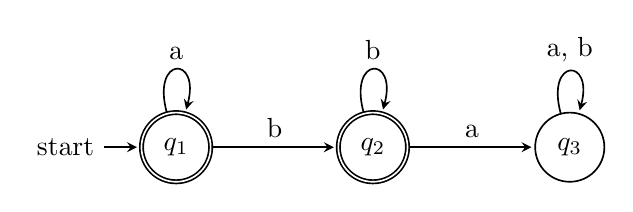
\begin{tikzpicture}[->,>=stealth,shorten >=1pt,auto,node distance=2.5cm, semithick]
      \node[state,initial, accepting] (q1) {$q_1$};
      \node[state, accepting] (q2) [right of=q1] {$q_2$};
      \node[state] (q3) [right of=q2] {$q_3$};

      \path (q1) edge [loop above] node {a} (q1)
            (q1) edge node {b} (q2)
            (q2) edge [loop above] node {b} (q2)
            (q2) edge node {a} (q3)
            (q3) edge [loop above] node {a, b} (q3)
            ;
    \end{tikzpicture}
\end{center}

\subsection{b) $\{w \mid w \text{ contains neither the substrings } ab \text{ nor } ba\}$}

The simpler language is $\{w \mid w \text{ contains } ab \text{ or } ba\}$.

DFA for the simpler language (contains $ab$ or $ba$):
\begin{center}
    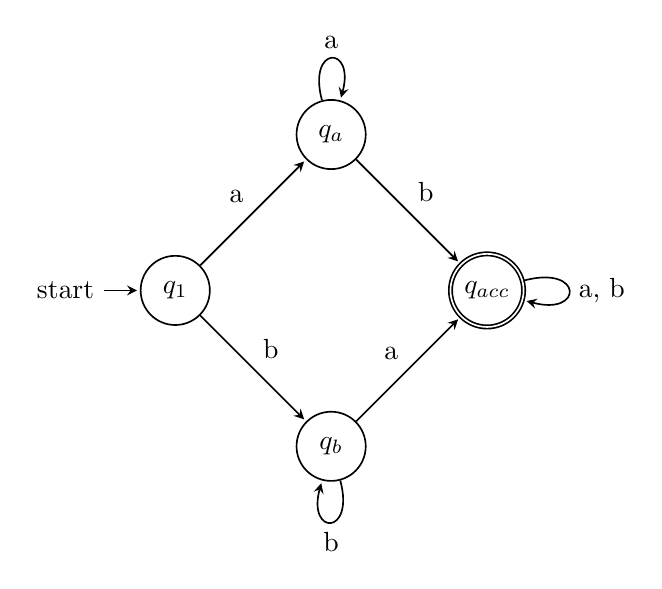
\begin{tikzpicture}[->,>=stealth,shorten >=1pt,auto,node distance=2.8cm, semithick]
      \node[state,initial] (q1) {$q_1$};
      \node[state] (qa) [above right of=q1] {$q_a$};
      \node[state] (qb) [below right of=q1] {$q_b$};
      \node[state, accepting] (qacc) [below right of=qa] {$q_{acc}$};

      \path (q1) edge node {a} (qa)
            (q1) edge node {b} (qb)
            (qa) edge [loop above] node {a} (qa)
            (qa) edge node {b} (qacc)
            (qb) edge [loop below] node {b} (qb)
            (qb) edge node {a} (qacc)
            (qacc) edge [loop right] node {a, b} (qacc)
            ;
    \end{tikzpicture}
\end{center}

DFA for the original language (contains neither $ab$ nor $ba$, i.e., $a^* \cup b^*$):
\begin{center}
    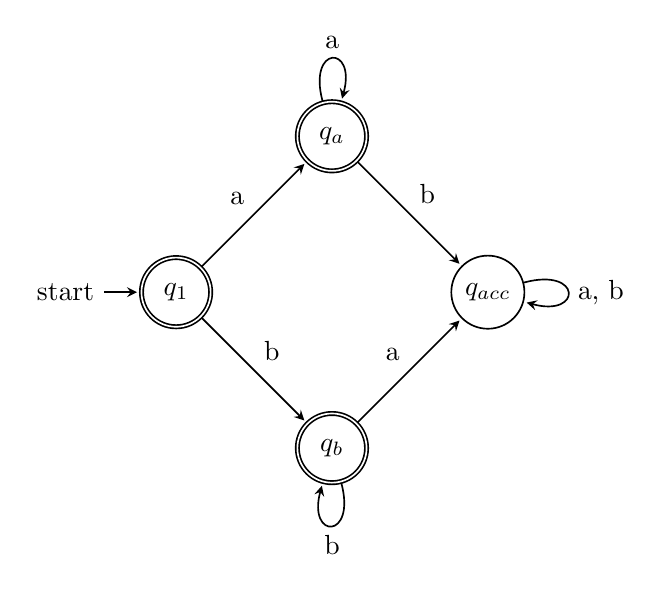
\begin{tikzpicture}[->,>=stealth,shorten >=1pt,auto,node distance=2.8cm, semithick]
      \node[state,initial, accepting] (q1) {$q_1$};
      \node[state, accepting] (qa) [above right of=q1] {$q_a$};
      \node[state, accepting] (qb) [below right of=q1] {$q_b$};
      \node[state] (qacc) [below right of=qa] {$q_{acc}$};

      \path (q1) edge node {a} (qa)
            (q1) edge node {b} (qb)
            (qa) edge [loop above] node {a} (qa)
            (qa) edge node {b} (qacc)
            (qb) edge [loop below] node {b} (qb)
            (qb) edge node {a} (qacc)
            (qacc) edge [loop right] node {a, b} (qacc)
            ;
    \end{tikzpicture}
\end{center}

\subsection{c) $\{w \mid w \text{ is any string not in } b^*a^*\}$}

The simpler language is $b^*a^*$ (zero or more $b$'s followed by zero or more $a$'s).

DFA for the simpler language ($b^*a^*$):
\begin{center}
    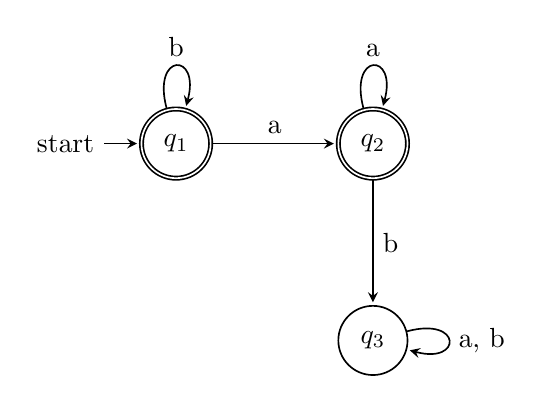
\begin{tikzpicture}[->,>=stealth,shorten >=1pt,auto,node distance=2.5cm, semithick]
      \node[state,initial, accepting] (q1) {$q_1$};
      \node[state, accepting] (q2) [right of=q1] {$q_2$};
      \node[state] (q3) [below of=q2] {$q_3$};

      \path (q1) edge [loop above] node {b} (q1)
            (q1) edge node {a} (q2)
            (q2) edge [loop above] node {a} (q2)
            (q2) edge node {b} (q3)
            (q3) edge [loop right] node {a, b} (q3)
            ;
    \end{tikzpicture}
\end{center}

DFA for the original language (not in $b^*a^*$, i.e., contains the substring $ba$):
\begin{center}
    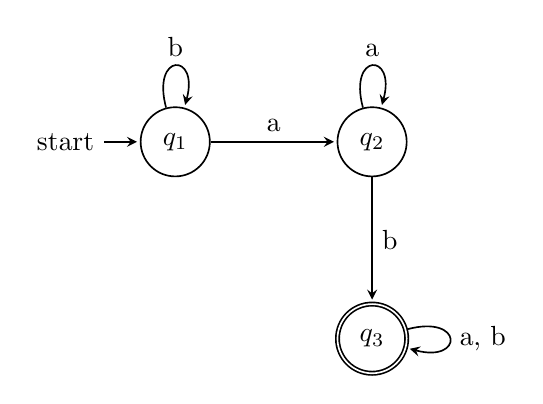
\begin{tikzpicture}[->,>=stealth,shorten >=1pt,auto,node distance=2.5cm, semithick]
      \node[state,initial] (q1) {$q_1$};
      \node[state] (q2) [right of=q1] {$q_2$};
      \node[state, accepting] (q3) [below of=q2] {$q_3$};

      \path (q1) edge [loop above] node {b} (q1)
            (q1) edge node {a} (q2)
            (q2) edge [loop above] node {a} (q2)
            (q2) edge node {b} (q3)
            (q3) edge [loop right] node {a, b} (q3)
            ;
    \end{tikzpicture}
\end{center}

\section{Question 6}

For each language, we construct DFAs for the two simpler languages, then use the product construction to obtain the DFA for their intersection.

\subsection{a) $\{w \mid w \text{ has at least two a's and at least three b's}\}$}

The simpler languages are:
\begin{itemize}
    \item $L_1 = \{w \mid w \text{ has at least two a's}\}$
    \item $L_2 = \{w \mid w \text{ has at least three b's}\}$
\end{itemize}

DFA for $L_1$ (at least two a's):
\begin{center}
    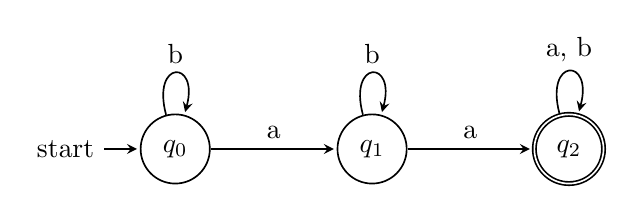
\begin{tikzpicture}[->,>=stealth,shorten >=1pt,auto,node distance=2.5cm, semithick]
      \node[state,initial] (q0) {$q_0$};
      \node[state] (q1) [right of=q0] {$q_1$};
      \node[state, accepting] (q2) [right of=q1] {$q_2$};

      \path (q0) edge [loop above] node {b} (q0)
            (q0) edge node {a} (q1)
            (q1) edge [loop above] node {b} (q1)
            (q1) edge node {a} (q2)
            (q2) edge [loop above] node {a, b} (q2)
            ;
    \end{tikzpicture}
\end{center}

DFA for $L_2$ (at least three b's):
\begin{center}
    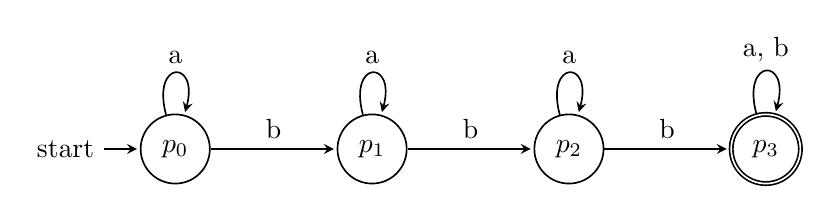
\begin{tikzpicture}[->,>=stealth,shorten >=1pt,auto,node distance=2.5cm, semithick]
      \node[state,initial] (p0) {$p_0$};
      \node[state] (p1) [right of=p0] {$p_1$};
      \node[state] (p2) [right of=p1] {$p_2$};
      \node[state, accepting] (p3) [right of=p2] {$p_3$};

      \path (p0) edge [loop above] node {a} (p0)
            (p0) edge node {b} (p1)
            (p1) edge [loop above] node {a} (p1)
            (p1) edge node {b} (p2)
            (p2) edge [loop above] node {a} (p2)
            (p2) edge node {b} (p3)
            (p3) edge [loop above] node {a, b} (p3)
            ;
    \end{tikzpicture}
\end{center}

DFA for $L_1 \cap L_2$ (product construction, accepting states are $(q_2, p_3)$):
\begin{center}
    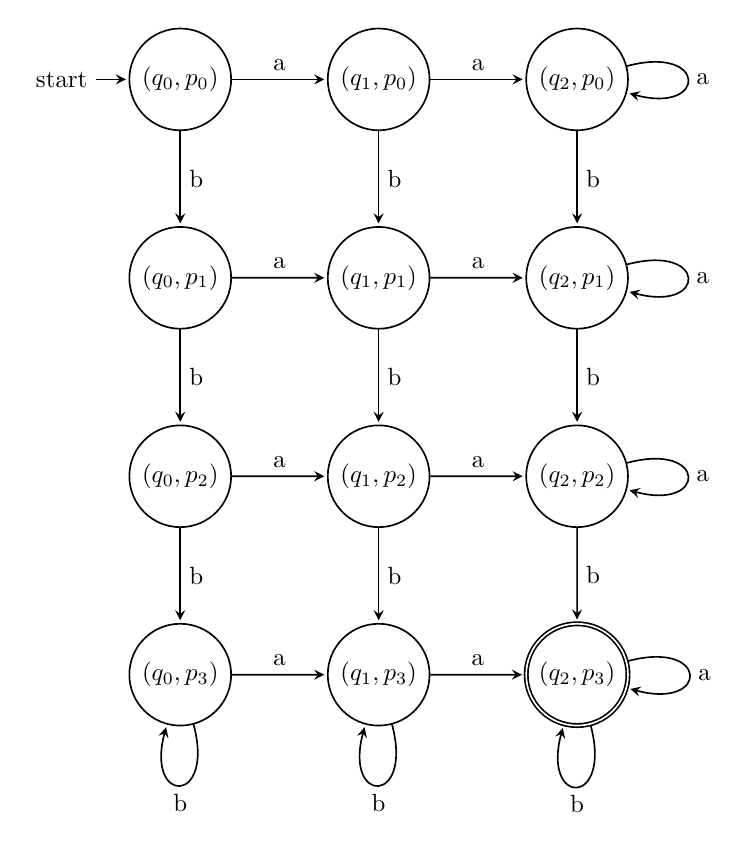
\begin{tikzpicture}[->,>=stealth,shorten >=1pt,auto,node distance=2.8cm, semithick, scale=0.9, transform shape]
      % Row p0 (0 b's)
      \node[state,initial] (q0p0) {$(q_0, p_0)$};
      \node[state] (q1p0) [right of=q0p0] {$(q_1, p_0)$};
      \node[state] (q2p0) [right of=q1p0] {$(q_2, p_0)$};
      
      % Row p1 (1 b)
      \node[state] (q0p1) [below of=q0p0] {$(q_0, p_1)$};
      \node[state] (q1p1) [right of=q0p1] {$(q_1, p_1)$};
      \node[state] (q2p1) [right of=q1p1] {$(q_2, p_1)$};
      
      % Row p2 (2 b's)
      \node[state] (q0p2) [below of=q0p1] {$(q_0, p_2)$};
      \node[state] (q1p2) [right of=q0p2] {$(q_1, p_2)$};
      \node[state] (q2p2) [right of=q1p2] {$(q_2, p_2)$};
      
      % Row p3 (3+ b's) - accepting for L2
      \node[state] (q0p3) [below of=q0p2] {$(q_0, p_3)$};
      \node[state] (q1p3) [right of=q0p3] {$(q_1, p_3)$};
      \node[state, accepting] (q2p3) [right of=q1p3] {$(q_2, p_3)$};

      % Transitions for a
      \path (q0p0) edge node {a} (q1p0)
            (q1p0) edge node {a} (q2p0)
            (q2p0) edge [loop right] node {a} (q2p0)
            (q0p1) edge node {a} (q1p1)
            (q1p1) edge node {a} (q2p1)
            (q2p1) edge [loop right] node {a} (q2p1)
            (q0p2) edge node {a} (q1p2)
            (q1p2) edge node {a} (q2p2)
            (q2p2) edge [loop right] node {a} (q2p2)
            (q0p3) edge node {a} (q1p3)
            (q1p3) edge node {a} (q2p3)
            (q2p3) edge [loop right] node {a} (q2p3)
            ;
            
      % Transitions for b
      \path (q0p0) edge node {b} (q0p1)
            (q0p1) edge node {b} (q0p2)
            (q0p2) edge node {b} (q0p3)
            (q0p3) edge [loop below] node {b} (q0p3)
            (q1p0) edge node {b} (q1p1)
            (q1p1) edge node {b} (q1p2)
            (q1p2) edge node {b} (q1p3)
            (q1p3) edge [loop below] node {b} (q1p3)
            (q2p0) edge node {b} (q2p1)
            (q2p1) edge node {b} (q2p2)
            (q2p2) edge node {b} (q2p3)
            (q2p3) edge [loop below] node {b} (q2p3)
            ;
    \end{tikzpicture}
\end{center}

\subsection{b) $\{w \mid w \text{ has an even number of a's and one or two b's}\}$}

The two simpler languages are:
\begin{itemize}
    \item $L_1 = \{w \mid w \text{ has an even number of a's}\}$
    \item $L_2 = \{w \mid w \text{ has one or two b's}\}$
\end{itemize}

The state diagrams for $L_1$: 
\begin{center}
    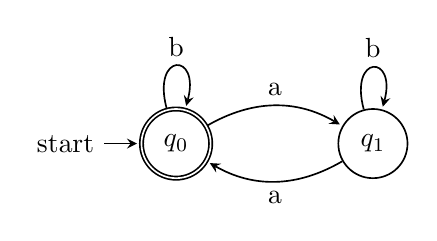
\begin{tikzpicture}[->,>=stealth,shorten >=1pt,auto,node distance=2.5cm, semithick]
      \node[state,initial, accepting] (q0) {$q_0$};
      \node[state] (q1) [right of=q0] {$q_1$};

      \path (q0) edge [bend left] node {a} (q1)
            (q0) edge [loop above] node {b} (q0)
            (q1) edge [bend left] node {a} (q0)
            (q1) edge [loop above] node {b} (q1)
            ;
    \end{tikzpicture}
\end{center}

The state diagram for $L_2$:
\begin{center}
    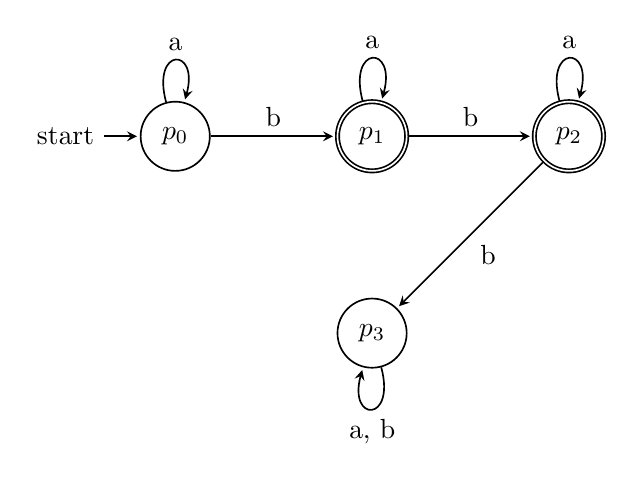
\begin{tikzpicture}[->,>=stealth,shorten >=1pt,auto,node distance=2.5cm, semithick]
      \node[state,initial] (p0) {$p_0$};
      \node[state, accepting] (p1) [right of=p0] {$p_1$};
      \node[state, accepting] (p2) [right of=p1] {$p_2$};
      \node[state] (p3) [below of=p1] {$p_3$};

      \path (p0) edge node {b} (p1)
            (p1) edge node {b} (p2)
            (p2) edge node {b} (p3)
            (p3) edge [loop below] node {a, b} (p3)
            (p0) edge [loop above] node {a} (p0)
            (p1) edge [loop above] node {a} (p1)
            (p2) edge [loop above] node {a} (p2)
            ;
    \end{tikzpicture}
\end{center}

Thus the intersection DFA (accepting states are $(q_0, p_1)$ and $(q_0, p_2)$):
\begin{center}
    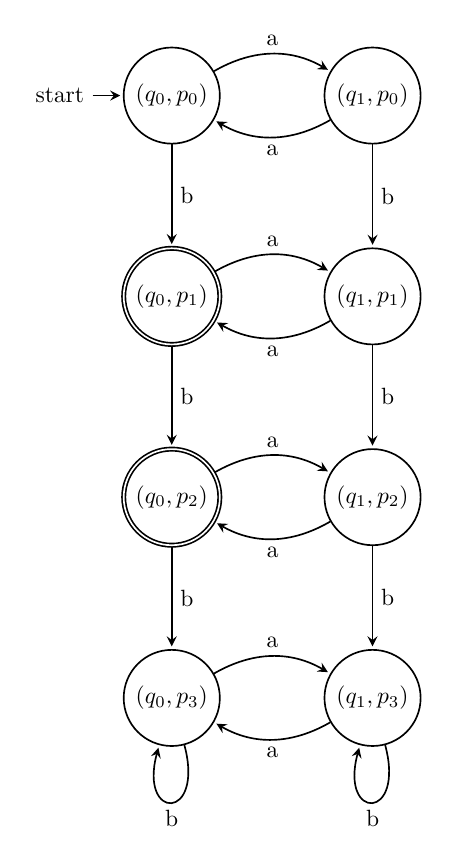
\begin{tikzpicture}[->,>=stealth,shorten >=1pt,auto,node distance=3cm, semithick, scale=0.85, transform shape]
      % Row p0 (0 b's)
      \node[state,initial] (q0p0) {$(q_0, p_0)$};
      \node[state] (q1p0) [right of=q0p0] {$(q_1, p_0)$};
      
      % Row p1 (1 b) - accepting for L2
      \node[state, accepting] (q0p1) [below of=q0p0] {$(q_0, p_1)$};
      \node[state] (q1p1) [right of=q0p1] {$(q_1, p_1)$};
      
      % Row p2 (2 b's) - accepting for L2
      \node[state, accepting] (q0p2) [below of=q0p1] {$(q_0, p_2)$};
      \node[state] (q1p2) [right of=q0p2] {$(q_1, p_2)$};
      
      % Row p3 (3+ b's) - trap for L2
      \node[state] (q0p3) [below of=q0p2] {$(q_0, p_3)$};
      \node[state] (q1p3) [right of=q0p3] {$(q_1, p_3)$};

      % Transitions for a (toggle between q0 and q1)
      \path (q0p0) edge [bend left] node {a} (q1p0)
            (q1p0) edge [bend left] node {a} (q0p0)
            (q0p1) edge [bend left] node {a} (q1p1)
            (q1p1) edge [bend left] node {a} (q0p1)
            (q0p2) edge [bend left] node {a} (q1p2)
            (q1p2) edge [bend left] node {a} (q0p2)
            (q0p3) edge [bend left] node {a} (q1p3)
            (q1p3) edge [bend left] node {a} (q0p3)
            ;
            
      % Transitions for b (move to next p state)
      \path (q0p0) edge node {b} (q0p1)
            (q0p1) edge node {b} (q0p2)
            (q0p2) edge node {b} (q0p3)
            (q0p3) edge [loop below] node {b} (q0p3)
            (q1p0) edge node {b} (q1p1)
            (q1p1) edge node {b} (q1p2)
            (q1p2) edge node {b} (q1p3)
            (q1p3) edge [loop below] node {b} (q1p3)
            ;
    \end{tikzpicture}
\end{center}

\subsection{c) $\{w \mid w \text{ starts with an a and has at most two b's}\}$}

The two simpler languages are:
\begin{itemize}
    \item $L_1 = \{w \mid w \text{ starts with an a}\}$
    \item $L_2 = \{w \mid w \text{ has at most two b's}\}$
\end{itemize}

The state diagram for $L_1$:
\begin{center}
    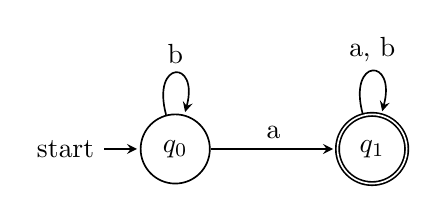
\begin{tikzpicture}[->,>=stealth,shorten >=1pt,auto,node distance=2.5cm, semithick]
      \node[state,initial] (q0) {$q_0$};
      \node[state, accepting] (q1) [right of=q0] {$q_1$};

      \path (q0) edge node {a} (q1)
            (q0) edge [loop above] node {b} (q0)
            (q1) edge [loop above] node {a, b} (q1)
            ;
    \end{tikzpicture}
\end{center}

The state diagram for $L_2$:
\begin{center}
    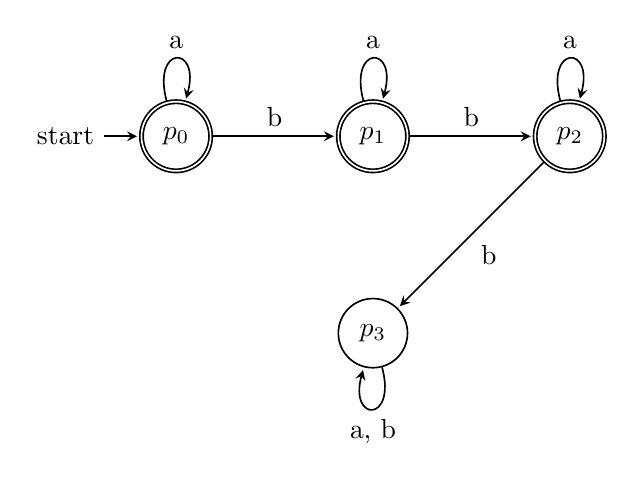
\begin{tikzpicture}[->,>=stealth,shorten >=1pt,auto,node distance=2.5cm, semithick]
      \node[state,initial,accepting] (p0) {$p_0$};
      \node[state,accepting] (p1) [right of=p0] {$p_1$};
      \node[state,accepting] (p2) [right of=p1] {$p_2$};
      \node[state] (p3) [below of=p1] {$p_3$};

      \path (p0) edge node {b} (p1)
            (p1) edge node {b} (p2)
            (p2) edge node {b} (p3)
            (p3) edge [loop below] node {a, b} (p3)
            (p0) edge [loop above] node {a} (p0)
            (p1) edge [loop above] node {a} (p1)
            (p2) edge [loop above] node {a} (p2)
            ;
    \end{tikzpicture}
\end{center}

Thus the intersection DFA (accepting states are $(q_1, p_0)$, $(q_1, p_1)$, and $(q_1, p_2)$):
\begin{center}
    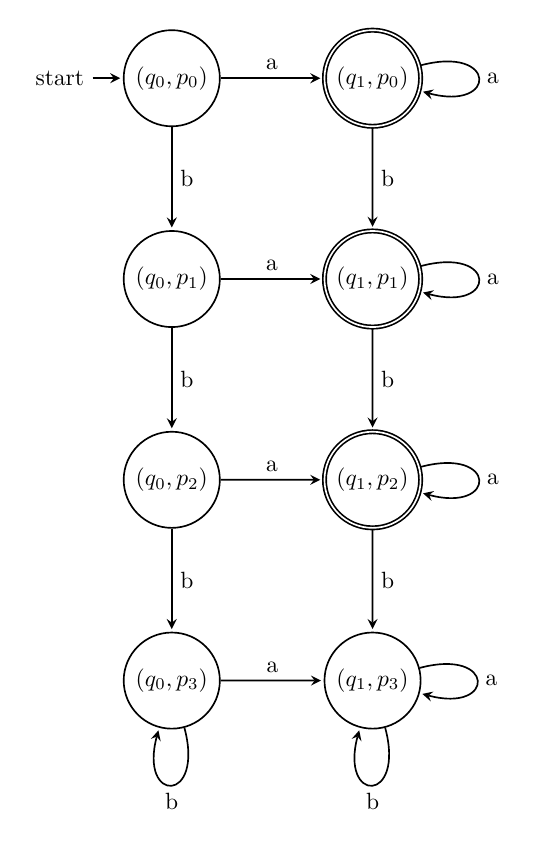
\begin{tikzpicture}[->,>=stealth,shorten >=1pt,auto,node distance=3cm, semithick, scale=0.85, transform shape]
      % Row p0 (0 b's)
      \node[state,initial] (q0p0) {$(q_0, p_0)$};
      \node[state, accepting] (q1p0) [right of=q0p0] {$(q_1, p_0)$};
      
      % Row p1 (1 b)
      \node[state] (q0p1) [below of=q0p0] {$(q_0, p_1)$};
      \node[state, accepting] (q1p1) [right of=q0p1] {$(q_1, p_1)$};
      
      % Row p2 (2 b's)
      \node[state] (q0p2) [below of=q0p1] {$(q_0, p_2)$};
      \node[state, accepting] (q1p2) [right of=q0p2] {$(q_1, p_2)$};
      
      % Row p3 (3+ b's) - trap for L2
      \node[state] (q0p3) [below of=q0p2] {$(q_0, p_3)$};
      \node[state] (q1p3) [right of=q0p3] {$(q_1, p_3)$};

      % Transitions for a
      \path (q0p0) edge node {a} (q1p0)
            (q1p0) edge [loop right] node {a} (q1p0)
            (q0p1) edge node {a} (q1p1)
            (q1p1) edge [loop right] node {a} (q1p1)
            (q0p2) edge node {a} (q1p2)
            (q1p2) edge [loop right] node {a} (q1p2)
            (q0p3) edge node {a} (q1p3)
            (q1p3) edge [loop right] node {a} (q1p3)
            ;
            
      % Transitions for b
      \path (q0p0) edge node {b} (q0p1)
            (q0p1) edge node {b} (q0p2)
            (q0p2) edge node {b} (q0p3)
            (q0p3) edge [loop below] node {b} (q0p3)
            (q1p0) edge node {b} (q1p1)
            (q1p1) edge node {b} (q1p2)
            (q1p2) edge node {b} (q1p3)
            (q1p3) edge [loop below] node {b} (q1p3)
            ;
    \end{tikzpicture}
\end{center}

\end{document}
